\documentclass[a4paper]{article}
\usepackage{float}
\usepackage[english]{babel}
\usepackage[utf8]{inputenc}
\usepackage{amsmath}
\usepackage{mathtools}
\usepackage{amsfonts}
\usepackage{caption}
\usepackage{subcaption}
\usepackage{graphicx}
\usepackage[colorinlistoftodos]{todonotes}
\usepackage{tcolorbox}
\usepackage{tikz}
\usepackage{lscape}
\usepackage{rotating}
\usepackage{listings}
\usepackage[colorlinks=true, allcolors=red]{hyperref}


\title{Assignment 2}

\author{Marcus Lindström \\ 880619-0453}

\date{\today}

\begin{document}
\setcounter{section}{2}
\maketitle
\subsection{Knowing the rules}
\vspace{10pt}
\subsubsection*{Question 2.1.1:}

\noindent Yes I have.

\subsubsection*{Question 2.1.2:}

\noindent I've not been collaborating with anyone regarding the problem formulations.

\subsubsection*{Question 2.1.3:}

\noindent No, I have not.

\subsection{Dependencies in a Directed Graphical Model}

\noindent For this part I chose to always assume that the colored nodes in the assignment pictures were unobserved i.e. $X_{r,c}^n$ in 2.2.4-2.2.6 and the set $X$ in 2.2.7-2.2.9, if the task does not explicitly state otherwise. 

\subsubsection*{Question 2.2.4:}
\noindent Yes.
\subsubsection*{Question 2.2.5:}
\noindent No.
\subsubsection*{Question 2.2.6:}
\noindent $A=\{ \mu_{r,c},\mu_{r+1,c},\mu_{r-1,c},\mu_{r,c+1},\mu_{r,c-1}\}$.
\subsubsection*{Question 2.2.7:}
\noindent No.
\subsubsection*{Question 2.2.8:}
\noindent No.
\subsubsection*{Question 2.2.9:}
\noindent $B = \{C^n:n\in [N]\}\cup \{Z^n_m:n\in [N],m\in [M]\}$.
\subsection{Likelihood of a tree GM}
\subsubsection*{Question 2.3.10:}
To calculate $P(\beta\vert T,\Theta)$, we first denote:
\begin{equation}
s(u,x_i)=P(x_{\downarrow u\cap L}\vert X_u = x_i),
\end{equation}

\noindent i.e. the probability of a subtree in $T$ rooted at $u$ given that $u$ has the value $x_i$. This is evaluated for all $u$ and $x_i$ recursively in a postorder fashion throughout the tree as follows:


\begin{align}
s(u,x_l)=\begin{cases}
1 \text{ if } x_u = x_l\\
0 \text{ otherwise}
\end{cases},\quad \forall u\in L,\\ 
s(u,x_i)=\prod_{v}\sum_{j}p(X_v=x_j\vert u=x_i) s(v,j),\quad \forall u\in V.
\end{align}

\noindent Where $\text{Pa}(v)=u$ and $x_l$ denotes the observed value of leaf $u$. These are stored in each tree node object as arrays with length $i$ (utilizing the concept of dynamical programming), and can then be used in order to compute 

\begin{equation}
P(\beta\vert T,\Theta)=\sum_{i}s(r,x_i)P(X_r=x_i).
\end{equation}

\noindent Where $r$ denotes the root.

\subsubsection*{Question 2.3.11:}
The likelihood computation was done for all trees given in the supplied data for all their respective samples resulting in the $27\times 3$ values listed in \autoref{table:likelihoods}. The code used to generate the likelihood of one tree was an adaption of the supplied code where a minor change was done to the Node class and also the inclusion of two more functions, these are supplied in appendix A. The function 'treeLikelihood' takes as a single input the tree root and generates the likelihood.
\newpage
\begin{landscape}
	
	\begin{table}[]
		\caption {Likelihood of the trees for different leaf set samples supplied in the assignment data.} \label{tab:title} 
		\centering
		\begin{tabular}{|l|l|l|l|}
			\hline
			\textbf{Tree Name\quad\textbackslash\quad Sample Number} & \textbf{1} & \textbf{2} & \textbf{3} \\ \hline
			tree\_k\_3\_md\_3\_mb\_7\_alpha\_{[}0.1 0.5 0.5{]} & 0.0155753676376 & 0.088023946612 & 0.132566342716 \\ \hline
			tree\_k\_2\_md\_5\_mb\_5\_alpha\_{[}0.5 0.5{]} & 9.54808310286e-09 & 1.70196002223e-08 & 1.98877723494e-08 \\ \hline
			tree\_k\_3\_md\_10\_mb\_2\_alpha\_{[}0.1 0.1 0.5{]} & 0.626315421676 & 0.0395215515401 & 0.626315421676 \\ \hline
			tree\_k\_3\_md\_3\_mb\_5\_alpha\_{[}0.1 0.1 0.5{]} & 0.980132424063 & 0.980132424063 & 0.980132424063 \\ \hline
			tree\_k\_2\_md\_10\_mb\_2\_alpha\_{[}0.1 0.5{]} & 0.887713912728 & 0.887713912728 & 0.887713912728 \\ \hline
			tree\_k\_5\_md\_3\_mb\_5\_alpha\_{[}1.  0.1 0.1 0.1 0.1{]} & 0.969178646303 & 0.969178646303 & 0.969178646303 \\ \hline
			tree\_k\_2\_md\_5\_mb\_7\_alpha\_{[}0.1 0.1{]} & 1.68177519885e-07 & 1.08421338523e-07 & 1.99629915369e-06 \\ \hline
			tree\_k\_5\_md\_10\_mb\_3\_alpha\_{[}0.1 0.1 1.  0.1 0.1{]} & 0.470978623571 & 0.470978623571 & 0.512871879451 \\ \hline
			tree\_k\_2\_md\_3\_mb\_5\_alpha\_{[}0.1 0.1{]} & 0.00313404991624 & 0.412272060248 & 0.412272060248 \\ \hline
			tree\_k\_3\_md\_5\_mb\_5\_alpha\_{[}0.1 0.5 0.1{]} & 0.0970490659887 & 0.0154784896316 & 0.551756975511 \\ \hline
			tree\_k\_5\_md\_5\_mb\_3\_alpha\_{[}0.1 0.1 0.1 0.1 0.1{]} & 0.0132414232261 & 0.000204224941913 & 0.00163860422448 \\ \hline
			tree\_k\_2\_md\_3\_mb\_3\_alpha\_{[}0.1 0.1{]} & 0.381008332013 & 0.381008332013 & 0.615008301187 \\ \hline
			tree\_k\_2\_md\_10\_mb\_4\_alpha\_{[}0.1 0.1{]} & 8.3402908101e-29 & 3.16982163034e-30 & 1.99587753423e-26 \\ \hline
			tree\_k\_2\_md\_5\_mb\_3\_alpha\_{[}0.1 0.1{]} & 0.00118320383767 & 0.0127382652232 & 0.0233906447948 \\ \hline
			tree\_k\_3\_md\_5\_mb\_3\_alpha\_{[}1.  1.  0.1{]} & 0.00942654885149 & 0.00116047367951 & 0.0034806316623 \\ \hline
			tree\_k\_5\_md\_5\_mb\_7\_alpha\_{[}0.1 0.1 0.1 0.5 0.1{]} & 3.55174184376e-33 & 3.51890290718e-29 & 1.11323090791e-35 \\ \hline
			tree\_k\_2\_md\_3\_mb\_7\_alpha\_{[}0.1 0.5{]} & 0.00138132794419 & 0.0244512198493 & 0.00229379539903 \\ \hline
			tree\_k\_3\_md\_5\_mb\_7\_alpha\_{[}0.5 0.1 0.1{]} & 4.08500834532e-43 & 8.96183860932e-46 & 5.44033353243e-50 \\ \hline
			tree\_k\_3\_md\_10\_mb\_4\_alpha\_{[}0.1 0.1 0.1{]} & 1.06182512223e-127 & 1.04982863414e-114 & 3.92169187603e-124 \\ \hline
			tree\_k\_5\_md\_3\_mb\_3\_alpha\_{[}0.1 0.5 0.1 0.1 0.1{]} & 0.227582214428 & 0.227582214428 & 0.174149077642 \\ \hline
			tree\_k\_3\_md\_3\_mb\_3\_alpha\_{[}0.1 1.  1. {]} & 0.27719738724 & 0.27719738724 & 0.111538941549 \\ \hline
			tree\_k\_5\_md\_10\_mb\_2\_alpha\_{[}1.  0.5 0.1 0.5 0.5{]} & 0.0405915901623 & 0.0372884579238 & 0.153115682736 \\ \hline
			tree\_k\_2\_md\_10\_mb\_3\_alpha\_{[}1.  0.1{]} & 0.150394889842 & 0.0177822750097 & 0.163041712878 \\ \hline
			tree\_k\_3\_md\_10\_mb\_3\_alpha\_{[}0.5 0.1 0.5{]} & 0.0637245109469 & 0.538856832905 & 0.309363515032 \\ \hline
			tree\_k\_5\_md\_3\_mb\_7\_alpha\_{[}0.1 0.1 0.5 1.  0.1{]} & 7.29290846901e-05 & 8.22304199798e-05 & 4.5918149222e-07 \\ \hline
			tree\_k\_5\_md\_10\_mb\_4\_alpha\_{[}0.1 0.1 0.1 0.1 0.1{]} & 2.44568054619e-299 & 6.06300242703e-289 & 8.74557857658e-304 \\ \hline
			tree\_k\_5\_md\_5\_mb\_5\_alpha\_{[}0.5 0.5 0.1 1.  1. {]} & 4.4826857152e-38 & 2.0737157063e-33 & 1.95182672736e-32 \\ \hline
		\end{tabular}
		\label{table:likelihoods}
	\end{table}
\end{landscape}

\section{Simple VI only for E level}

\subsubsection*{Question 2.4.12:}

The VI-algorithm to approximate the posterior was implemented in python with code supplied in appendix B.

\subsubsection*{Question 2.4.13:}

The exact posterior is given by a Gaussian-Gamma distribution $\mathcal{NG}(\mu,\tau\vert \mu_n, \lambda_n, a_n, b_n)$ where

\begin{align}
&\mu_n=\frac{\lambda_0\mu_0 + n\bar{x}}{\lambda_0+n},\\
&\lambda_n = \lambda_0+n,\\
&a_n=a_0+n/2,\\
&b_n=b_0+\frac{1}{2}\bigg(\sum_{i=1}^{n}(x_i-\bar{x})^2+\frac{\lambda_0n(\bar{x}-\mu_0)^2}{(\lambda_0+n)}\bigg).
\end{align}

\noindent It is derived from realizing that it is proportional to the likelihood times the prior and that the used prior is conjugate, then identifying all parameters after some rearrangement. A full derivation can be found \href{https://www.cs.ubc.ca/~murphyk/Papers/bayesGauss.pdf}{here} for example.  

\subsubsection*{Question 2.4.14:}

Below follows three cases where approximate posterior distributions $p(\mu,\tau\vert \mathbf{X})$ were inferred using VI until convergence. In each case, different parameter setups were used to tweak both the $\tau$-priors and also the data generating normal distribution. 

\vspace{8pt}

\textbf{Case 1:} 
\begin{itemize}
	\item Prior: $a_0=1$, $b_0=0.001$, $\lambda_0=1$, $\mu_0 = 0$
	\item Data: $\mu=0$, $\tau=1$
\end{itemize}

\begin{figure*}[h!]
	\centering
	\begin{subfigure}[t]{0.5\textwidth}
		\centering
		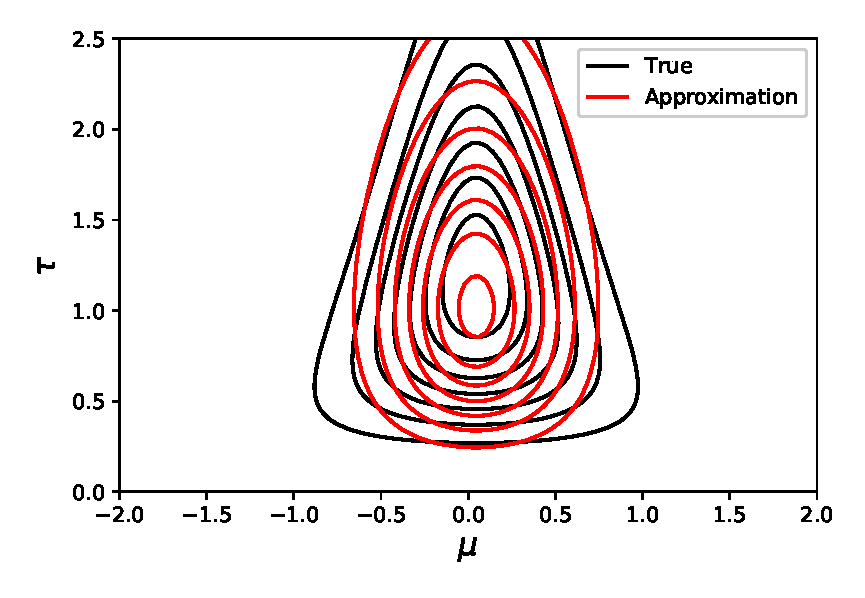
\includegraphics[height=1.5in]{Case1a.eps}
		\caption{$n=5$}
	\end{subfigure}%
	~ 
	\begin{subfigure}[t]{0.5\textwidth}
		\centering
		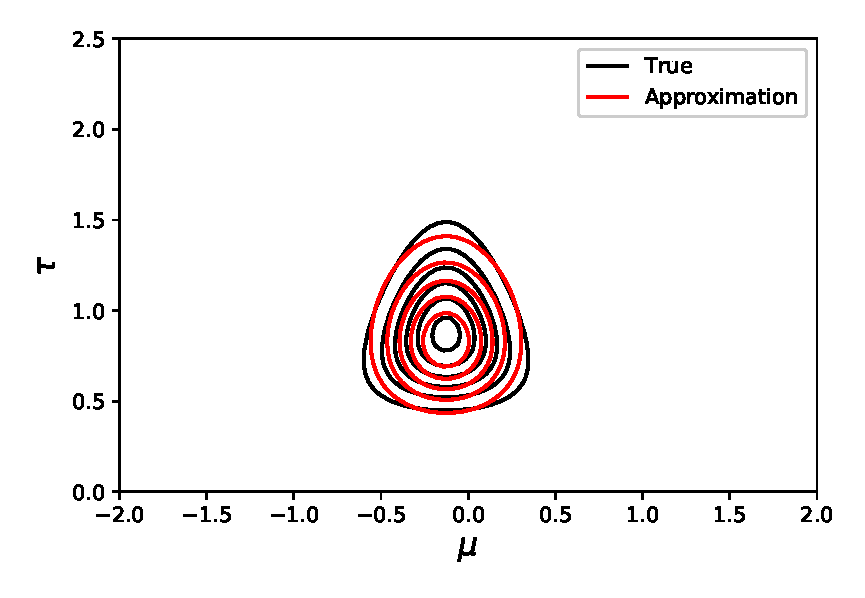
\includegraphics[height=1.5in]{Case1b.eps}
		\caption{$n=20$}
	\end{subfigure}
	\caption{Comparison of the true and approximate posterior for case 1.}
\end{figure*}
\newpage
\textbf{Case 2:} 
\begin{itemize}
	\item Prior: $a_0=1$, $b_0= 0.001$, $\lambda_0=1$, $\mu_0 = 0$
	\item Data: $\mu=4$, $\tau=1$
\end{itemize}

\begin{figure*}[h!]
	\centering
	\begin{subfigure}[t]{0.5\textwidth}
		\centering
		\includegraphics[height=1.5in]{Case2a.eps}
		\caption{$n=5$}
	\end{subfigure}%
	~ 
	\begin{subfigure}[t]{0.5\textwidth}
		\centering
		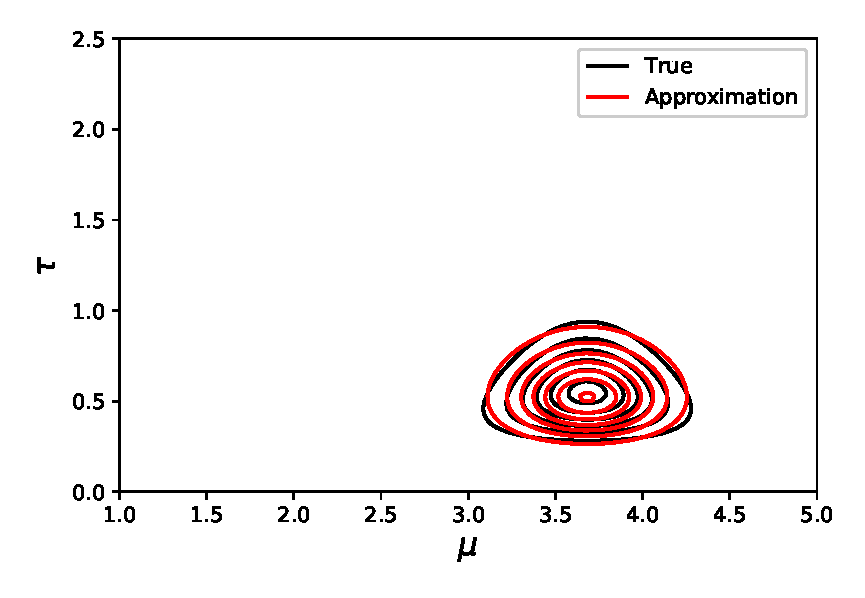
\includegraphics[height=1.5in]{Case2b.eps}
		\caption{$n=20$}
	\end{subfigure}
	\caption{Comparison of the true and approximate posterior for case 2.}
\end{figure*}

\textbf{Case 3:} 
\begin{itemize}
	\item Prior: $a_0=20$, $b_0= 10$, $\lambda_0=1$, $\mu_0 = 0$
	\item Data: $\mu=0$, $\tau=1$
\end{itemize}

\begin{figure*}[h!]
	\centering
	\begin{subfigure}[t]{0.5\textwidth}
		\centering
		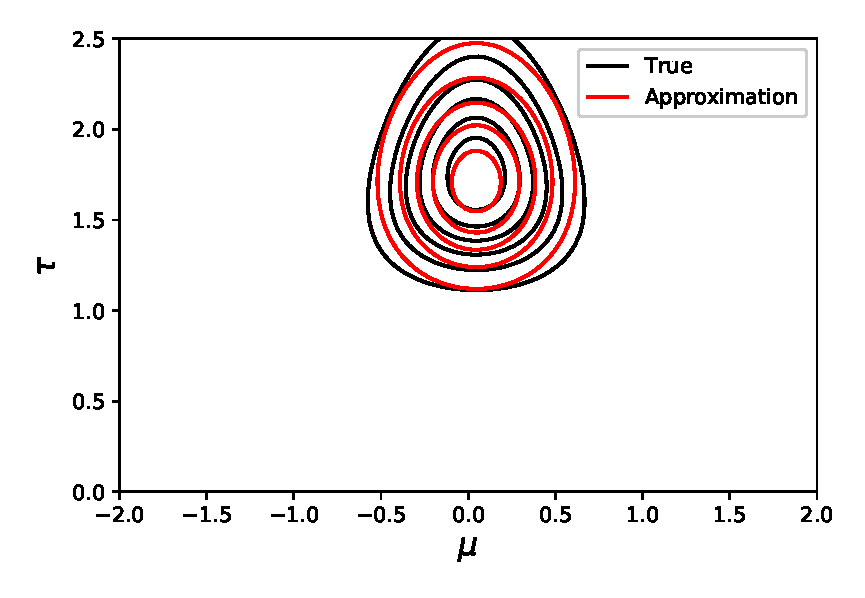
\includegraphics[height=1.5in]{Case3a.eps}
		\caption{$n=5$}
	\end{subfigure}%
	~ 
	\begin{subfigure}[t]{0.5\textwidth}
		\centering
		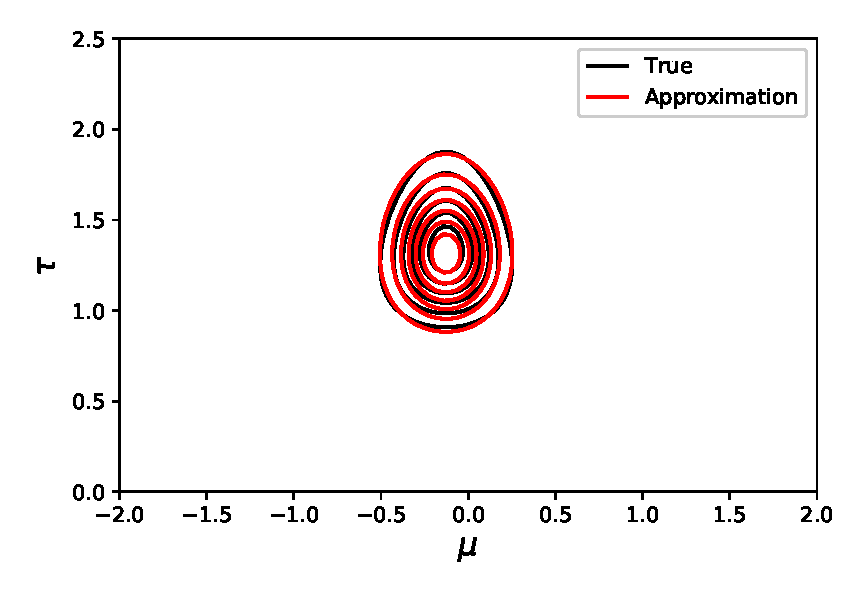
\includegraphics[height=1.5in]{Case3b.eps}
		\caption{$n=20$}
	\end{subfigure}
	\caption{Comparison of the true and approximate posterior for case 3.}
\end{figure*}

\noindent We see that in both case 1 and 2 the true posterior and the approximate (somewhat) catches the parameters accurately whereas case 1 is closest, (note also that the same random seed was used in all cases). This is due to how we encode our prior belief in the parameters, case 1 had a better "guess" of the data mean encoded in its prior, which however mostly affect the learned precision value. This is partly a consequence of the distribution being constrained to a finite probability mass and has to become more compact in one direction if it's to stretch in another. 

If we look at figure \ref{fig:Gamma}, we see how the precision Gamma-prior was modeled in case 1 \& 2 compared to case 3. The formers were modeled with the least informative prior, and adding more data was indeed informative, which we can see as the distribution becoming more compact. Case 3 used a considerably more informative prior, placing much of its probability mass on a wrong value. Adding fifteen more data samples did not do as much in terms of providing more information compared to earlier cases, which suggests slower (at least initial) learning rates.

The approximate posterior mean always coincides with that of the true one, which does not come as a surprise since they are given by the same expression. 

It's also apparent that the true posterior does no factorize in a way used in the VI-algorithm, this is easiest to see in case 1 \& 2 where they differ quite a lot. The approximate is also more compact in each case, which is a general result of factorized variational approximations of posterior distributions according to Bishop p. 467. 

\begin{figure*}[h!]
	\centering
	\begin{subfigure}[t]{0.5\textwidth}
		\centering
		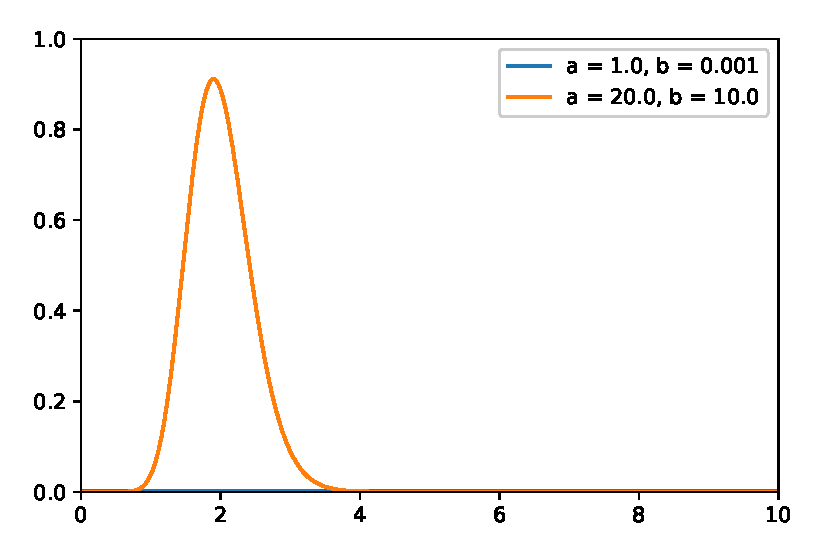
\includegraphics[height=1.5in]{Gamma1.eps}
	\end{subfigure}%
	~ 
	\begin{subfigure}[t]{0.5\textwidth}
		\centering
		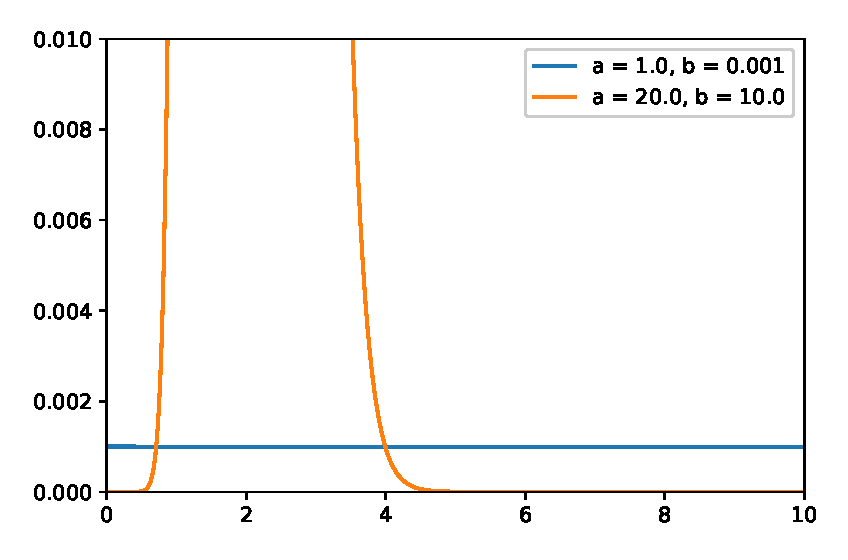
\includegraphics[height=1.5in]{Gamma2.eps}
	\end{subfigure}
	\caption{\label{fig:Gamma}Comparison of the two types of Gamma-priors used, the right picture is a zoomed in version of the left.}
\end{figure*}
\newpage
\appendix
\section{Code for 2.3}
\lstinputlisting[language=Python]{code.py}
\newpage
\section{Code for 2.4}
\lstinputlisting[language=Python]{Code2.4.py}
\end{document}